\section[تمرین اول - سؤال سوم: خوشه‌بندی سلسله‌مراتب]
{\faProjectDiagram\ \ تمرین اول ـ سؤال سوم: خوشه‌بندی داده‌های IRIS با الگوریتم Agglomerative Clustering}

\begin{stepbox}

\field{هدف و معرفی مسئله}{
هدف این بخش، پیاده‌سازی و ارزیابی الگوریتم خوشه‌بندی سلسله‌مراتب تجمعی (\lr{Agglomerative Hierarchical Clustering}) روی مجموعه داده معروف \lr{IRIS} بود. این مجموعه داده شامل ۱۵۰ نمونه از سه گونه مختلف گل زنبق (\lr{Setosa}، \lr{Versicolor} و \lr{Virginica}) بر اساس ۴ ویژگی طول و عرض کاسبرگ و گلبرگ است.

در این تمرین، فرآیند خوشه‌بندی به صورت کاملاً بدون نظارت (\lr{Unsupervised}) و با حذف برچسب‌های واقعی کلاس‌ها انجام شد تا توانایی الگوریتم در کشف ساختار طبیعی داده‌ها سنجیده شود.
}

\field{تحلیل داده‌ها و بصری‌سازی اولیه}{
ابتدا داده‌های مربوط به هر یک از سه گونه گل به صورت مجزا فیلتر شده و توزیع ویژگی‌های آن‌ها بررسی گردید. سپس جهت مقایسه اولیه، نمودار پراکندگی ۲ بعدی نمونه‌ها بر اساس طول و عرض کاسبرگ برای تمامی کلاس‌های واقعی ترسیم شد.

\vspace{0.4cm}

\begin{center}
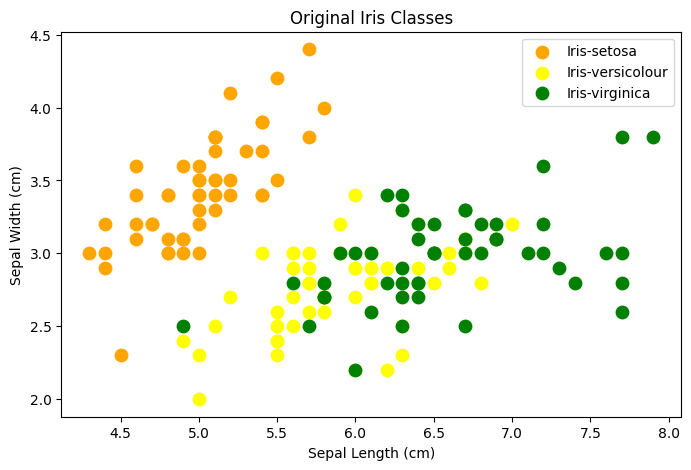
\includegraphics[width=.72\textwidth]{images/iris_original_classes.png}
\captionof{figure}{پراکندگی واقعی گونه‌های مختلف گل \lr{IRIS} در فضای ۲ بعدی}
\label{fig:iris_original}
\end{center}
}

\field{تحلیل دندروگرام و تعیین نوع پیوند (Linkage)}{
برای تعیین نحوه ادغام خوشه‌ها، دندروگرام مربوط به داده‌ها با چهار روش پیوند مختلف شامل \lr{Single} ،\lr{Complete} ،\lr{Average} و \lr{Median} رسم گردید. دندروگرام یک نمودار درختی است که نحوه ادغام تدریجی داده‌ها را در فواصل مختلف نشان می‌دهد.

بر اساس ساختار دندروگرام و دانش اولیه از مسئله، تعداد خوشه‌ها برابر با

\[
k = 3
\]

تعیین شد و معیارهای پیوند میان خوشه‌ها ارزیابی گردیدند که روش \lr{Average Linkage} بهترین پایداری و تفکیک‌پذیری را نشان داد.

\vspace{0.4cm}

\begin{center}
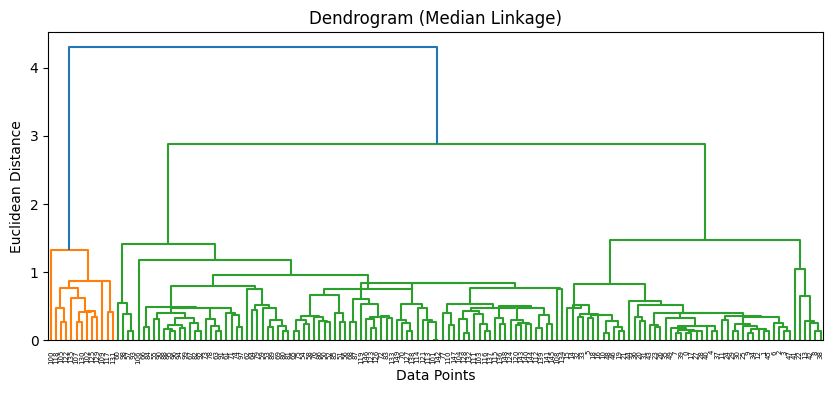
\includegraphics[width=.80\textwidth]{images/dendrogram_linkages.png}
\captionof{figure}{نمودار دندروگرام حاصل از خوشه‌بندی سلسله‌مراتب روی داده‌های \lr{IRIS}}
\label{fig:dendrogram}
\end{center}
}

\field{اجرای الگوریتم و ارزیابی با ضریب سیلوئت}{
مدل \lr{AgglomerativeClustering} با تعیین $n\_clusters=3$ و نوع پیوند \lr{average} روی ویژگی‌های داده اجرا شد. جهت ارزیابی کیفیت خوشه‌بندی، معیار **ضریب سیلوئت (\lr{Silhouette Score})** محاسبه گردید.

مقدار ضریب سیلوئت به‌دست‌آمده برابر است با:

\[
\boxed{\text{Silhouette Score} \approx 0.55}
\]

این مقدار مثبت و نسبتاً بالا نشان‌دهنده ساختار مناسب خوشه‌ها و جدایش قابل‌قبول آن‌ها از یکدیگر است.

\vspace{0.4cm}

\begin{center}
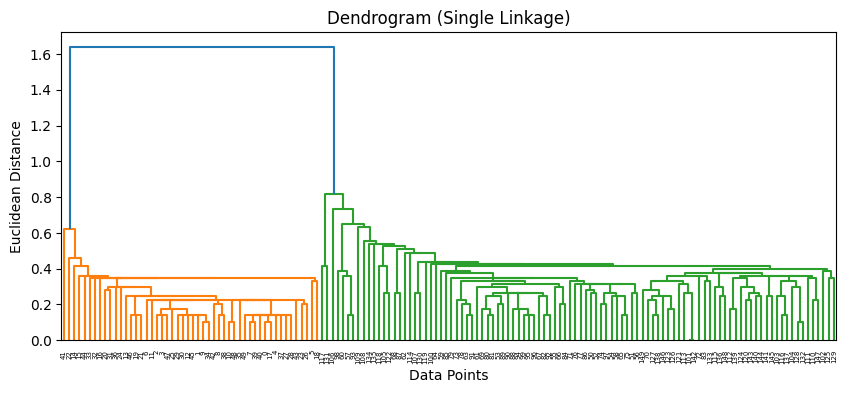
\includegraphics[width=.72\textwidth]{images/hierarchical_clusters_result.png}
\captionof{figure}{نتایج حاصل از خوشه‌بندی داده‌های \lr{IRIS} توسط الگوریتم \lr{Agglomerative Clustering}}
\label{fig:hierarchical_result}
\end{center}
}

\field{نتایج و تحلیل مقایسه‌ای}{
تحلیل و مقایسه خوشه‌های تشکیل‌شده توسط الگوریتم با برچسب‌های واقعی داده‌ها نتایج زیر را نشان می‌دهد:

\begin{itemize}
\item **گونه \lr{Setosa}:** به دلیل فاصله زیاد ویژگی‌های آن از دو گونه دیگر، به صورت کاملاً مجزا و با دقت $100\%$ در یک خوشه مستقل قرار گرفت.
\item **گونه‌های \lr{Versicolor} و \lr{Virginica}:** به دلیل همپوشانی طیف ویژگی‌های ظاهری در برخی نمونه‌ها، مرز میان این دو گونه دارای اندکی تداخل است که در خروجی الگوریتم خوشه‌بندی نیز این همپوشانی به خوبی مشهود می‌باشد.
\end{itemize}
}

\field{جمع‌بندی}{
در این بخش الگوریتم خوشه‌بندی سلسله‌مراتب روی مجموعه داده \lr{IRIS} پیاده‌سازی شد. با تحلیل نمودار دندروگرام و اعمال روش پیوند \lr{Average}، الگوریتم موفق شد بدون دسترسی به برچسب‌های واقعی، سه خوشه اصلی داده‌ها را با ضریب سیلوئت $0.55$ بازسازی کند. نتایج نشان داد که خوشه‌بندی سلسله‌مراتب گزینه‌ای بسیار مناسب برای درک ساختار درختی و ارتباطات میان داده‌ها است.
}

\end{stepbox}